\documentclass[11pt]{article}
\usepackage{ghb}

% Restored from WordPress post 612 on 2026-10-21.
% Original URL: https://nicknash.me/2018/04/07/speculating-about-store-buffer-capacity/
% Main plot redrawn from the author's surviving CSV.
% Missing baseline and VTune screenshots replaced with historical observations.
% Corrected Peterson/Dekker, the direction of the reorder bound, retirement
% versus draining, and the qualification on coalescing and the extra entry.
\title{Speculating About Store-Buffer Capacity}
\date{2018-04-07}
\summary{Exposing the store-buffer}
\begin{document}

\section{Removing Fences}

If you're ever looking to squeeze the performance of lock-free code it's tempting to try and get rid of unnecessary memory fences. On x86/x64, this can be tantalising: for ordinary loads and stores to normal, write-back memory, the reordering we need to worry about at the processor level is an earlier store being overtaken by a later load from another address.

So on such architectures the question arises: are there thread-safe data structures where we can do without even a store-load fence?

For coordinating just two threads, the answer is of course yes. A single-producer, single-consumer queue can, for example, use acquire-release operations without an explicit store-load fence on x86. But what about more generally?

The answer turns out to also be yes, as shown in the ASPLOS 2014 paper \href{https://www.cs.tau.ac.il/~mad/publications/asplos2014-ffwsq.pdf}{Fence-Free Work Stealing on Bounded TSO Processors}.

Doing this requires determining the ``reorder bound'' of the processor in question, which is closely related to the capacity of its \emph{store buffer}. In this post, I'm going to describe and reproduce an experiment the paper uses that allows us to infer the store-buffer capacity of an Intel processor.

\section{A Tiny Bit of Background}

So what are store buffers and why do processors have them? One reason is that processors are typically \emph{speculative}, meaning that they will execute instructions before it is certain those instructions are actually required. This is enabled by \emph{branch prediction}, which roughly amounts to the processor guessing ahead of time which way an if-statement will go.

One type of instruction that makes speculation tricky is a store to memory. If the store in question turns out not to be required after all, then the processor would need to somehow undo the store in memory. That would be bad enough, but making a speculative store visible to other processors would make programming such a machine hell.

The solution is to have stores first write into the store buffer, and only later ``drain'' to the cache, once they are no longer speculative and the required cache-coherence conditions are met. Buffering also lets execution continue while a store waits to become globally visible.

A useful distinction here is between \emph{retiring} a store from the reorder buffer and \emph{draining} it from the store buffer. A store can have retired and still occupy a store-buffer entry. Retirement alone does not free that entry.

\section{Store Buffers Meet Memory Models}

In the x86 memory model, it's the store buffer that allows an earlier store to appear reordered with a subsequent load from another address. This famously makes Peterson's mutex and Dekker's algorithm incorrect without suitable memory ordering. A minimal demonstration based on Intel's memory-ordering white paper is \href{https://github.com/nicknash/StoreLoad}{here}.

The store buffer has finite capacity. Subject to the coalescing wrinkle we'll return to at the end, that limits the number of \emph{earlier stores a load can overtake}. For Haswell, Intel's \emph{64 and IA-32 Architectures Optimization Reference Manual} documents 42 store-buffer entries.

\section{An Experiment}

Enough background! How can we indirectly observe the store-buffer capacity? Well, Intel includes this warning in the optimisation manual:

\begin{quote}
As long as the store does not complete, its entry remains occupied in the store buffer. When the store buffer becomes full, new micro-ops cannot enter the execution pipe and execution might stall.
\end{quote}

So the start of the idea is to repeatedly execute a sequence of $S$ stores, vary $S$, and compute the average time per iteration. In pseudocode:

\begin{verbatim}
for S = 1 to 100
    Record StartTime
    repeat N times
        Perform S stores
    Record EndTime
    Report (EndTime - StartTime) / N
\end{verbatim}

This doesn't give much away about the store buffer. In my original run, the timing curve showed no useful cliff at its capacity: consecutive iterations keep issuing stores, so the loop runs into a sustained throughput limit instead of starting each batch with an empty buffer. The graph from that first run has been lost.

A simple way to give the store buffer time to drain is to execute a stream of other instructions after the stores. Even no-ops will do:

\begin{verbatim}
for S = 1 to 100
    Record StartTime
    repeat N times
        Perform S stores
        Perform 500 no-ops
    Record EndTime
    Report (EndTime - StartTime) / N
\end{verbatim}

The actual implementation generates an unrolled sequence of stores to distinct, adjacent locations followed by 500 no-ops. The surviving CSV covers $S=0$ through $79$; the pseudocode above just gives the shape of the experiment.

What now happens is quite interesting. While there are remaining store-buffer entries, some of the time spent processing the no-ops can overlap the stores. No-ops don't really execute on an execution port: Haswell eliminates them in the renamer. But they still consume front-end bandwidth, at up to four per cycle.

What about when we attempt a store where no store-buffer entry is available?

To get a read on that we can again refer to our trusty optimisation manual. Its description of the renamer includes the following:

\begin{quote}
The Renamer is the bridge between the in-order part [...] and the dataflow world of the Scheduler. It moves up to four micro-ops every cycle from the micro-op queue to the out-of-order engine.
\end{quote}

As well as performing register renaming, it allocates resources to micro-ops, including load and store buffers.

So it really \emph{seems} that if a store-buffer entry isn't available, the store in question won't proceed past allocation. More importantly, the subsequent no-ops cannot pass it either. Some of the work that previously overlapped the stores now has to wait.

On my Haswell, this is the result I saw:

\begin{figure}[ht]
\centering
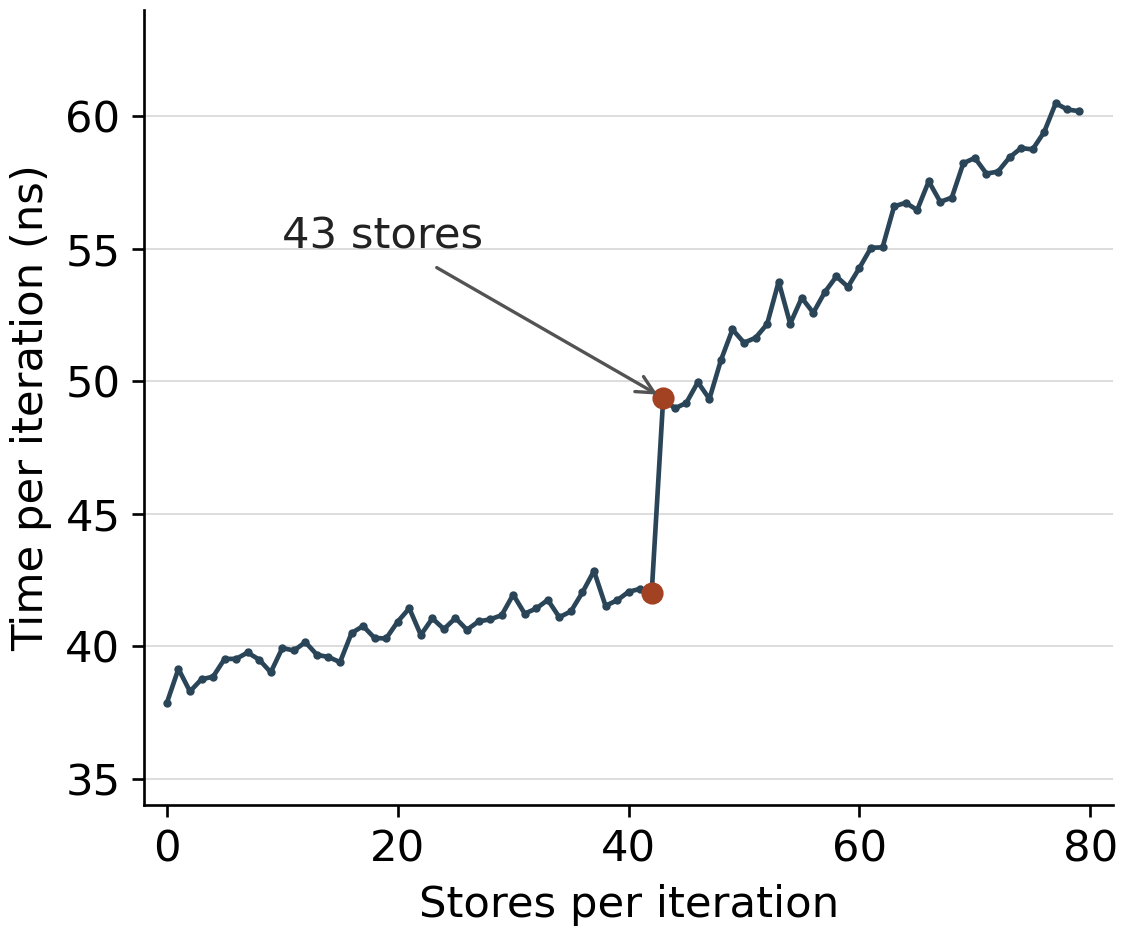
\includegraphics[width=\linewidth,alt={Original Haswell timings with 500 no-ops per iteration. Time rises gently to 42.01 nanoseconds at 42 stores then jumps to 49.37 nanoseconds at 43 stores.}]{assets/store-buffer/haswell-500-nops.png}
\caption{Redrawn from the original measurements, with microseconds converted to nanoseconds. Each iteration includes 500 no-ops.}
\end{figure}

The jump appears when 43 stores are attempted: from about 42.01 to 49.37 nanoseconds per iteration. Haswell's documented store-buffer capacity is 42. The subsequent rise is consistent with additional stores waiting for entries to become available, though the timing curve alone doesn't establish every pipeline detail.

So that's it! A timing experiment has exposed a boundary consistent with the 42-entry store buffer. Of course, nothing is stopping us from measuring a bit more directly.

\section{Measuring}

To get some independent evidence that this behaviour is a result of store-buffer stalls, we can crank out VTune. The relevant event is \texttt{RESOURCE\_STALLS.SB}. Intel describes it as counting cycles stalled because the pipeline has reached its store-resource limit; the stall ends when a store commits its data to cache or memory.

For 42 stores on my Haswell, the \texttt{RESOURCE\_STALLS.SB} row was clean as a whistle. Changing things to 43 stores showed store-buffer stalls, just as we'd expect. That was a second, not-very-surprising (but satisfying!) check that store-buffer entries were being exhausted.

\emph{Restoration note: the two VTune screenshots have not been recovered. The observations above are retained from the original post; the surviving CSV contains timings, not performance-counter readings.}

I also checked what Intel's Architecture Code Analyzer, IACA, had to say about a loop kernel of 42 versus 43 stores followed by a stream of no-ops. It seemed not to simulate enough of the microarchitecture to report anything interesting here. For completeness, the repository retains the \href{https://github.com/nicknash/GuessStoreBuffer/blob/master/iaca-42-stores-throughput.log}{42-store throughput report} and \href{https://github.com/nicknash/GuessStoreBuffer/blob/master/iaca-42-stores-trace.log}{pipeline trace}, as well as the \href{https://github.com/nicknash/GuessStoreBuffer/blob/master/iaca-43-stores-throughput.log}{43-store report} and \href{https://github.com/nicknash/GuessStoreBuffer/blob/master/iaca-43-stores-trace.log}{trace}. They do let you see the four no-ops per cycle running in parallel with the stores, though.

\section{Conclusion}

If you'd like to explore the experiment, you can find the \href{https://github.com/nicknash/GuessStoreBuffer}{code} and \href{https://github.com/nicknash/GuessStoreBuffer/blob/master/results-500-nop.csv}{original measurements} on GitHub. It's a fairly hilarious/horrible setup: a C\# program generates a C++ program with the required assembly instructions inside it!

Lastly, although the experiment gives us a store-buffer capacity, it doesn't by itself nail down the processor's reorder bound. Consecutive stores to the same location may be coalesced, allowing more stores than the entry count suggests to remain unseen by another core. The \href{https://www.cs.tau.ac.il/~mad/publications/asplos2014-ffwsq.pdf}{paper's Section 7.3} investigates this separately, infers an additional buffering stage, and derives a bound one greater than the measured capacity when its software avoids coalescing. That qualification matters: ``capacity plus one'' is not a general rule we can read straight off this graph.

\end{document}
